\documentclass{aucklandthesis}

%%%%%%%%%%%%%%%%%%%%%%%%%%%%%%%%%%%%%%%%%%%%%%%%%%%%%%%%%%%%%%%
% Add any LaTeX packages and other preamble here if required
%%%%%%%%%%%%%%%%%%%%%%%%%%%%%%%%%%%%%%%%%%%%%%%%%%%%%%%%%%%%%%%

\author{ZHAOMING SU}
\title{Time Series Visualisation for Auckland Air Quality}
\degrees{Bachelor of Science (Honours) in Statistics}
\supervisor{Dr.~Earo Wang}
\cosupervisor{Prof.~Chris Wild}
\def\degreetitle{}
% Add subject and keywords below
\hypersetup{
     %pdfsubject={The Subject},
     %pdfkeywords={Some Keywords},
     pdfauthor={ZHAOMING SU},
     pdftitle={Time Series Visualisation for Auckland Air Quality},
     pdfproducer={Bookdown with LaTeX}
}


\bibliography{thesisrefs}

\begin{document}

\pagenumbering{roman}

\titlepage

{\setstretch{1.2}\rm\tighttoc\doublespacing}

\hypertarget{abstract}{%
\chapter*{Abstract}\label{abstract}}
\addcontentsline{toc}{chapter}{Abstract}

The abstract should outline the main approach and findings of the thesis and must not be more than 500 words.

\newpage

\hypertarget{acknowledgements}{%
\chapter*{Acknowledgements}\label{acknowledgements}}
\addcontentsline{toc}{chapter}{Acknowledgements}

I would like to thank my pet goldfish for \dots

\hypertarget{copyright-notice}{%
\chapter*{Copyright notice}\label{copyright-notice}}
\addcontentsline{toc}{chapter}{Copyright notice}

\textcopyright { } \authorname~(\number\the\year).

I certify that I have made all reasonable efforts to secure copyright permissions for third-party content included in this thesis and have not knowingly added copyright content to my work without the owner's permission.

\newpage

\emph{(Standard thesis)}

This thesis is an original work of my research and contains no material which has been accepted for the award of any other degree or diploma at any university or equivalent institution and that, to the best of my knowledge and belief, this thesis contains no material previously published or written by another person, except where due reference is made in the text of the thesis.

\emph{(Thesis including published works declaration)}

I hereby declare that this thesis contains no material which has been accepted for the award of any other degree or diploma at any university or equivalent institution and that, to the best of my knowledge and belief, this thesis contains no material previously published or written by another person, except where due reference is made in the text of the thesis.

This thesis includes (insert number) original papers published in peer reviewed journals and (insert number) submitted publications. The core theme of the thesis is (insert theme). The ideas, development and writing up of all the papers in the thesis were the principal responsibility of myself, the student, working within the (insert name of academic unit) under the supervision of (insert name of supervisor).

(The inclusion of co-authors reflects the fact that the work came from active collaboration between researchers and acknowledges input into team-based research.) Remove this paragraph for theses with sole-authored work

In the case of (insert chapter numbers) my contribution to the work involved the following:

I have / have not renumbered sections of submitted or published papers in order to generate a consistent presentation within the thesis.

\begin{table}
\centering\footnotesize\tabcolsep=0.12cm
\begin{tabular}{|p{1.2cm}|p{2cm}|p{1.8cm}|p{3.4cm}|p{3.5cm}|p{1.5cm}|}
\hline
\RaggedRight\textbf{Thesis chapter}  & 
\RaggedRight\textbf{Publication title}  & 
\RaggedRight\textbf{Status (published, in press, accepted or returned for revision)}  &  
\RaggedRight\textbf{Nature and \% of student contribution} & 
\RaggedRight\textbf{Co-author name(s), nature and \% of co-author’s contribution} &  \RaggedRight\textbf{Co-author(s), Monash student Y/N} \\ 
\hline
2 & xx & xx  & xx & xx & \multicolumn{1}{c|}{N}   \\
\hline
3 & xx & xx  & xx & xx  & \multicolumn{1}{c|}{N}   \\
\hline
4 & xx & xx  & xx & xx & \multicolumn{1}{c|}{N}    \\
\hline
5 & xx & xx  & xx & xx & \multicolumn{1}{c|}{N}   \\
\hline
\end{tabular}
\end{table}

\textbf{Student name:} \authorname

\textbf{Student signature:}

\textbf{Date:}

\hypertarget{preface}{%
\chapter*{Preface}\label{preface}}
\addcontentsline{toc}{chapter}{Preface}

The material in Chapter \ref{ch:intro} has been submitted to the journal \emph{Journal of Impossible Results} for possible publication.

The contribution in Chapter \ref{ch:litreview} of this thesis was presented in the International Symposium on Nonsense held in Dublin, Ireland, in July 2015.

\clearpage\pagenumbering{arabic}\setcounter{page}{0}

\hypertarget{ch:intro}{%
\chapter{Introduction (Template Demo)}\label{ch:intro}}

This is where you introduce the main ideas of your thesis, and an overview of the context and background.

In a PhD, Chapter 2 would normally contain a literature review. Typically, Chapters 3--5 would contain your own contributions. Think of each of these as potential papers to be submitted to journals. Finally, Chapter 6 provides some concluding remarks, discussion, ideas for future research, and so on. Appendixes can contain additional material that don't fit into any chapters, but that you want to put on record. For example, additional tables, output, etc.

\hypertarget{rmarkdown}{%
\section{Rmarkdown}\label{rmarkdown}}

In this template, the rest of the chapter shows how to use Rmarkdown. The big advantage of using Rmarkdown is that it allows you to include your R code directly into your thesis, to ensure there are no errors in copying and pasting, and that everything is reproducible. It also helps you stay better organized.

For details on using \emph{R Markdown} see \url{http://rmarkdown.rstudio.com}.

\hypertarget{data}{%
\section{Data}\label{data}}

Included in this template is a file called \texttt{sales.csv}. This contains quarterly data on Sales and Advertising budget for a small company over the period 1981--2005. It also contains the GDP (gross domestic product) over the same period. All series have been adjusted for inflation. We can load in this data set using the following command:

\begin{Shaded}
\begin{Highlighting}[]
\NormalTok{sales <-}\StringTok{ }\KeywordTok{ts}\NormalTok{(}\KeywordTok{read.csv}\NormalTok{(}\StringTok{"data/sales.csv"}\NormalTok{)[, }\DecValTok{-1}\NormalTok{], }\DataTypeTok{start =} \DecValTok{1981}\NormalTok{, }\DataTypeTok{frequency =} \DecValTok{4}\NormalTok{)}
\end{Highlighting}
\end{Shaded}

Any data you use in your thesis can go into the data directory. The data should be in exactly the format you obtained it. Do no editing or manipulation of the data outside of R. Any data munging should be scripted in R and form part of your thesis files (possibly hidden in the output).

\hypertarget{figures}{%
\section{Figures}\label{figures}}

Figure \ref{fig:deaths} shows time plots of the data we just loaded. Notice how figure captions and references work. Chunk names can be used as figure labels with \texttt{fig:} prefixed. Never manually type figure numbers, as they can change when you add or delete figures. This way, the figure numbering is always correct.

\begin{figure}
\centering
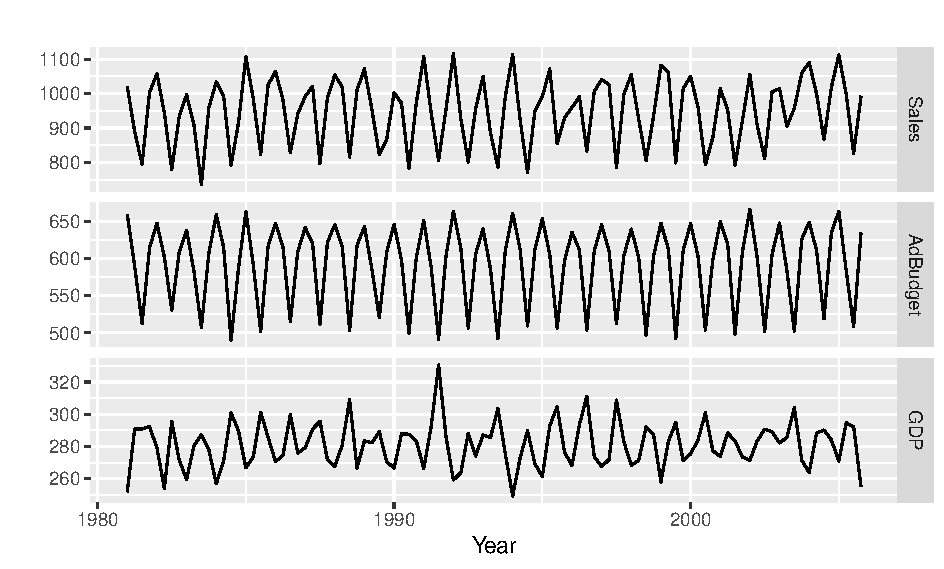
\includegraphics{thesis_files/figure-latex/deaths-1.pdf}
\caption{\label{fig:deaths}Quarterly sales, advertising and GDP data.}
\end{figure}

\hypertarget{results-from-analyses}{%
\section{Results from analyses}\label{results-from-analyses}}

We can fit a dynamic regression model to the sales data.

If \(y_t\) denotes the sales in quarter \(t\), \(x_t\) denotes the corresponding advertising budget and \(z_t\) denotes the GDP, then the resulting model is:
\begin{equation}
  y_t - y_{t-4} = \beta (x_t-x_{t-4}) + \gamma (z_t-z_{t-4}) + \theta_1 \varepsilon_{t-1} + \Theta_1 \varepsilon_{t-4} + \varepsilon_t
\end{equation}
where
\(\beta = 2.28\),
\(\gamma = 0.97\),
\(\theta_1 = NA\),
and
\(\Theta_1 = -0.90\).

\hypertarget{tables}{%
\section{Tables}\label{tables}}

Let's assume future advertising spend and GDP are at the current levels. Then forecasts for the next year are given in Table \ref{tab:salesforecasts}.

\begin{table}[ht]
\begin{center}
\begin{tabular}{lllll}
\toprule
Point Forecast & Lo 80 & Hi 80 & Lo 95 & Hi 95 \\
\midrule
1000.2 &  947.7 & 1052.7 & 919.9 & 1080.5 \\
1013.1 &  959.3 & 1066.8 & 930.9 & 1095.3 \\
1076.7 & 1022.9 & 1130.6 & 994.4 & 1159.0 \\
1003.5 &  949.7 & 1057.4 & 921.2 & 1085.8 \\
\bottomrule
\end{tabular}
\caption{Forecasts for the next year assuming Advertising budget and GDP are unchanged.}
\label{tab:salesforecasts}
\end{center}
\end{table}

Again, notice the use of labels and references to automatically generate Table numbers. In this case, we need to generate the label ourselves.

The \texttt{knitLatex} package is useful for generating tables from R output. Other packages can do similar things including the \texttt{kable} function in \texttt{knitr} which is somewhat simpler but you have less control over the result. If you use \texttt{knitLatex} to generate tables, don't forget to include \texttt{results="asis"} in the chunk settings.

\hypertarget{ch:litreview}{%
\chapter{Literature Review (Draft)}\label{ch:litreview}}

\hypertarget{sec:expsmooth}{%
\section{Exponential smoothing (Template Demo)}\label{sec:expsmooth}}

Exponential smoothing was originally developed in the late 1950s \autocite{Brown59,Brown63,Holt57,Winters60}. Because of their computational simplicity and interpretability, they became widely used in practice.

Empirical studies by \textcite{MH79} and \textcite{Metal82} found little difference in forecast accuracy between exponential smoothing and ARIMA models. This made the family of exponential smoothing procedures an attractive proposition \autocite[see][]{CKOS01}.

The methods were less popular in academic circles until \textcite{OKS97} introduced a state space formulation of some of the methods, which was extended in \textcite{HKSG02} to cover the full range of exponential smoothing methods.

\hypertarget{ch:data}{%
\chapter{The Auckland Environmental Data}\label{ch:data}}

\hypertarget{sec:intro}{%
\section{Introduction}\label{sec:intro}}

The data, provided by \textcite{aklenvdata}, includes data on 14 parameters from 10 monitoring stations in Auckland from as North as Takapuna to as South as Patumahoe. Parameters consist of air quality index (AQI), 10 pollutant levels and four other meteorological variables, reported in hourly resolution, with various starting dates (since as early as 2003 in Takapuna) until April 2021. All time-stamps are in New Zealand Standard Time (UTC+12) to avoid duplicated index upon boundaries of daylight saving.

\begin{center}
\begin{longtable}{lll}
\toprule
Parameter & Unit & Note \\
\midrule
\endhead
\caption{Parameters available in the data.}\\
\bottomrule
\endfoot
AQI &  & Air Quality Index \\
BC(370) & ngm\textsuperscript{-3} & Black carbon at 370nm wavelength \\
BC(880) & ngm\textsuperscript{-3} & Black carbon at 880nm wavelength \\
NO & \textmu gm\textsuperscript{-3} & Nitrogen monoxide concentration \\
NO\textsubscript{2} & \textmu gm\textsuperscript{-3} & Nitrogen dioxide concentration \\
NOx & \textmu gm\textsuperscript{-3} & Nitrogen oxides concentration \\
PM2.5 & \textmu gm\textsuperscript{-3} & Particulate matter with diameter <2.5\textmu m \\
PM10 & \textmu gm\textsuperscript{-3} & Particulate matter with diameter <10\textmu m \\
SO\textsubscript{2} & \textmu gm\textsuperscript{-3} & Sulphur dioxide concentration \\
O\textsubscript{3} & \textmu gm\textsuperscript{-3} & Ozone concentration \\
CO & mgm\textsuperscript{-3} & Carbon monoxide concentration \\
Relative Humidity & \% &  \\
Temperature & $^{\circ}$C &  \\
Wind Speed & ms\textsuperscript{-1} &  \\
Wind Direction & $^{\circ}$ &  \\
AQI Level of Concern &  & Derived from AQI \\
\label{tab:datasummary}
\end{longtable}
\end{center}

\hypertarget{sec:clean}{%
\section{Data Cleaning}\label{sec:clean}}

The final data set is composed of two separate data sets, each with a different data structure. Cleaning and manipulation are needed for ensuring the consistency of format for combination. The desired structure of the final data consists of observations, each uniquely identified by the date-time and location serving as the index and key, with records of all parameters.

The environmental parameter data set is in long format, with each observation consisting of a single record of one parameter. In total, there are 7,461,261 records from 10 locations with 14 parameters in the data set. Preliminary inspection finds that 4,654 records (0.06\% of total) have a missing time-stamp and 60,312 records (0.81\%) have missing value. Besides, 104,332 records are found to have a negative value. Nevertheless, all pollutants are reported in units in the form of mass per unit volume, and other parameters except for temperature are only sensible if positive \autocite{airunit}. Thus, 104,257 records of insensible negative values are removed. Of the 7,292,038 time-and-numerically sensible records, 239,374 (3.28\%) are duplicate with 120,207 redundant records. Further checking reveals that 230,822 of the duplicates have inconsistent values. However, as the scale of the inconsistency of most duplicate records is small, the first-appearing records of duplicates are kept. The cleaned data set consists of 7,171,831 (96.12\%) valid records with 719,640 records (10.03\%) of implicit time gaps.

The parameter wind direction is from a differently structured data set, with each observation consisting of wind direction records of all locations uniquely identified by a date-time stamp. Of the seven locations of interest (locations also in the environmental data set), the data set includes 940,632 records with 207,436 (22.05\%) missing values but no implicit time gaps. It is worth noting that 39,193 records (4.17\%) have an inconsistent format for their time-stamp.

The clean data set consists of 1,138,535 observations and 18 variables (date-time as the index, location as the key, 15 original parameters and one derived parameter) from Jun 1, 2003, to Apr 30, 2021. The time range is different for each location, with Customs St as short as since Jan 1, 2020. After accounting for all implicit time gaps, 9,173,003 records have missing values, implying a real missing rate of 53.71\%. It is noteworthy that extreme values from input error are more frequent in the earlier years. The final data set is subsetted from the year 2016.

\appendix

\hypertarget{additional-stuff}{%
\chapter{Additional stuff}\label{additional-stuff}}

You might put some computer output here, or maybe additional tables.

Note that line 5 must appear before your first appendix. But other appendices can just start like any other chapter.

\printbibliography[heading=bibintoc]



\end{document}
